\documentclass{article}
\usepackage{url,graphicx}
\title{A Test for ODT generation in LaTeXML}
\author{Michael Kohlhase\\Jacobs University\\\url{m.kohlhase@jacobs-university.de}}
\date{\today}
\begin{document}
\maketitle

\section{Purpose (Heading 1)}

The following sections illustrate various possibilities in ODF Text.

\subsection{A simple series of paragraphs (Heading 2)}

This section contains a series of paragraphs.

This is a second paragraph.

And a third paragraph.

\subsection{A section with lists (Heading 2)}
Elements to illustrate:
\begin{itemize}
\item hyperlinks
\item italics and bold text
\item lists (ordered and unordered)
\end{itemize}
How to figure out ODF
\begin{enumerate}
\item work out the content.xml tags
\item  work styles into the mix
\item  figure out how to apply what we learned to spreadsheets and presentations
\end{enumerate}
The URL for Flickr is \url{http://www.flickr.com}.  The API page is \url{http://www.flickr.com/services/api/}

\section{A Table (Heading 1)}
\begin{tabular}{|l|l|l|}\hline
  Website & Description & URL \\\hline
  Flickr & A social photo sharing site & \url{http://www.flickr.com}\\\hline 
  Google Maps & An online map & \url{http://maps.google.com}\\\hline
\end{tabular}

\section{Footnotes (Heading 1)}

This sentence has an accompanying footnote.\footnote{You are reading a footnote.}   And
another one \footnote{another footnote}. 

\section{An Image}
 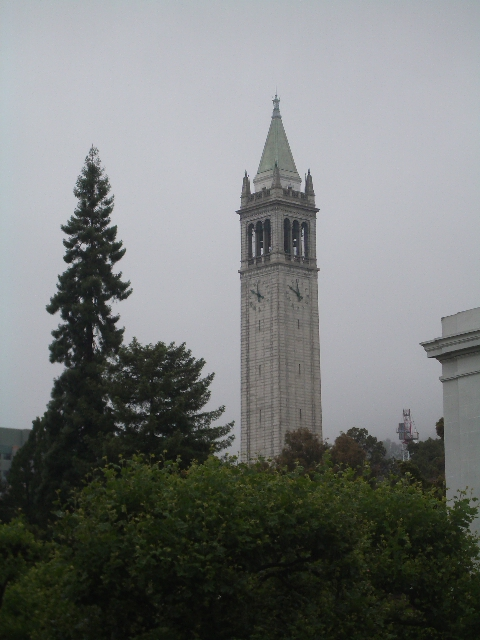
\includegraphics[width=9cm]{campanile_fog}

\section{A Figure}

\begin{figure}[ht]
  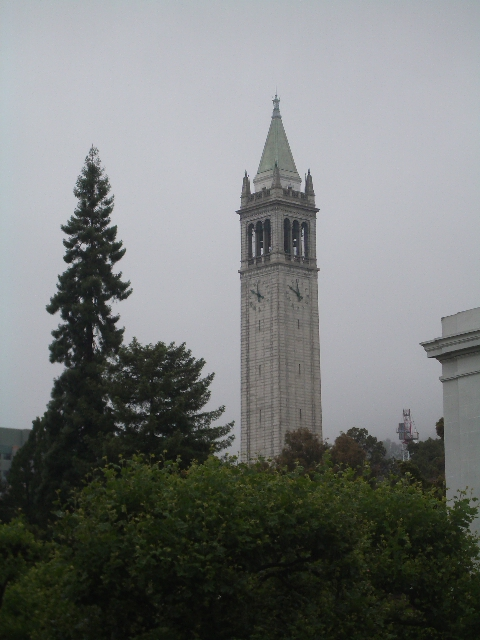
\includegraphics[width=9cm]{campanile_fog}
  \caption{Testing a Figure}
\end{figure}

\section{Citations}
a first citation \cite{aaa} and a second one \cite{bbb}

\section{Some Math}
some inline math: $a2+2ab+b^2$ and an equation 
\begin{equation}
  x = -b\pm \frac{\sqrt{b^2-4ac}}{2a}
\end{equation}
\bibliographystyle{alpha}
\bibliography{test}
\end{document}
